\documentclass[12pt]{article}
\usepackage{graphicx}
\usepackage{subfig}
\usepackage{hyperref}
\usepackage{float}
\usepackage[margin=1in]{geometry}

\title{CarND Behavioral Cloning Project Writeup}
\author{Tiffany Huang}
\date{\today}

\begin{document}
\maketitle


\section{Behavioral Cloning Project}
This project consists on the following steps/tasks:
\begin{itemize}
\item {Use the simulator to collect data of good driving behavior.}
\item {Build, a convolution neural network in Keras that predicts steering angles from images.}
\item {Train and validate the model with a training and validation set.}
\item {Test that the model successfully drives around track one without leaving the road.}
\item {Summarize the results in a written report.}
\end{itemize}
My project code can be found here: \url{https://github.com/tahuang/Behavioral_Cloning}. Next, I will consider each of the rubric points individually and describe how I addressed each point in my implementation.

\section{Files Submitted \& Code Quality}
My project includes the following files:
\begin{itemize}
\item {\texttt{model.py} containing the script to create and train the model}
\item {\texttt{drive.py} for driving the car in autonomous mode}
\item {\texttt{model.h5} containing the trained convolutional neural network}
\item {\texttt{writeup\_report.pdf} summarizing the results}
\end{itemize}

Using the Udacity provided simulator and my drive.py file, the car can be driven autonomously around the track by executing: \texttt{python drive.py model.h5}.

The \texttt{model.py} file contains the code for training and saving the convolutional neural network. The file shows the pipeline I used for training and validating the model, and it contains comments to explain how the code works.

\section{Model Architecture and Training Strategy}
\subsection{Final Model Architecture}
My final model is outlined in lines 83-95 of \texttt{model.py}. Preprocessing of the data is done with normalization of the images using a Keras lambda layer (line 78). The input images are also cropped to remove irrelevant pixels in the driving images that could distract the model (line 80). The final model consists of the following layers:
\begin{center}
\begin{tabular}{|c|p{10cm}|}
\hline
\textbf{Layer} & \textbf{Description} \\
\hline
Input & 160 x 320 x 3 RGB Image \\
\hline
Convolutional & 24 5 x 5 filters, 2 x 2 stride, VALID padding, ReLU activation \\
\hline
Convolutional & 36 5 x 5 filters, 2 x 2 stride, VALID padding, ReLU activation \\
\hline
Convolutional & 48 5 x 5 filters, 2 x 2 stride, VALID padding, ReLU activation \\
\hline
Convolutional & 64 3 x 3 filters, 1 x 1 stride, VALID padding, ReLU activation \\
\hline
Convolutional & 64 3 x 3 filters, 1 x 1 stride, VALID padding, ReLU activation \\
\hline
Flatten & \\
\hline
Fully Connected & Outputs 100 x 1\\
\hline
Dropout & Drop 0.2 (one fifth) of samples \\
\hline
Fully Connected & Outputs 50 x 1\\
\hline
Dropout & Drop 0.2 (one fifth) of samples \\
\hline
Fully Connected & Outputs 10 x 1\\
\hline
Dropout & Drop 0.2 (one fifth) of samples \\
\hline
Fully Connected & Outputs 1 x 1 \\
\hline
\end{tabular}
\end{center}

\subsection{Attempts to Reduce Overfitting}
The model contains dropout layers in order to reduce overfitting (lines 90, 92, 94). The model was tested by running it through the simulator and ensuring that the vehicle stayed on the track for at least one lap. 
\subsection{Model Parameter Tuning}
The model used an Adam optimizer, so the learning rate was not tuned manually (line 97). 
\subsection{Appropriate Training Data}
Training data was chosen to keep the vehicle on the road. I used a combination of center lane driving and recovering from the left and right sides of the road. More details can be found in the next section.

\section{Model Architecture \& Training Strategy}
\subsection{Solution Design Approach}
The overall strategy for deriving a model architecture was to try some well-known architectures and tweak them to get the car successfully driving around the track. My first step was to use a covolutional neural network similar to LeNet[1] since we've used it before as a basis for the Traffic Sign Classifier project. This model could be appropriate because the inputs in this problem are also RGB images and it's a powerful network that has proven successful for various tasks.

In order to gauge how well the model was working, I split my image and steering angle data into a training and validation set. I found that my first model had a low mean squared error on the training set but a high mean squared error on the validation set. This implied that the model was overfitting.

To combat the overfitting, I modified the model by adding a few dropout layers between the fully connected layers near the end of the network. However, the car was still struggling with certain sections so I decided to try the even more powerful Nvidia architecture[2] because this architecture has been used for very similar applications before, namely driving a car autonomously.

After changing the network architecture, I kept the dropout layers to reduce overfitting. However, there were still some spots on the track where the vehicle was driving off the road where there was no barrier. To improve the driving behavior in these cases, I added more training data to reinforce staying on the road. I flipped the left and right camera images in addition to the center ones to increase the amount of data and I recorded 2 more laps of driving including some driving where I am recovering back to the center of the road from the left or right side.

After adding more training data, performance significantly improved. There was still a small case where the car would roll up on the ledge on the section of the road with red and white stripes on the sides in the right turn after the bridge. To improve this behavior, I tuned the steering angle correction for the left and right side camera images. 

At the end of the process, the vehicle can drive autonomously around the track without leaving the road!

\subsection{Creation of the Training Set \& Training Process}
To capture good driving behavior, I first recorded one lap around the track using center lane driving. Here is an example of center lane driving:
\begin{figure}[h]
\centering
\includegraphics[scale = 1]{data3/IMG/center_2017_11_29_20_11_58_441.jpg}
\caption{Center lane driving}
\end{figure}

After a few iterations of building my network, I recorded 2 more laps around the track and also recorded the vehicle recovering from the left and right side of the track. Here's some examples of recoveries from the side of the track:
\begin{figure}[h]
\centering
\includegraphics[scale = 1]{data3/IMG/center_2017_12_21_20_08_10_962.jpg}
\caption{Recovery from left side part 1}
\end{figure}

\begin{figure}[h]
\centering
\includegraphics[scale = 1]{data3/IMG/center_2017_12_21_20_08_11_370.jpg}
\caption{Recovery from left side part 2}
\end{figure}

\begin{figure}[h]
\centering
\includegraphics[scale = 1]{data3/IMG/center_2017_12_21_20_08_11_643.jpg}
\caption{Recovery from left side part 3}
\end{figure}

\begin{figure}[h]
\centering
\includegraphics[scale = 1]{data3/IMG/center_2017_12_21_20_08_14_315.jpg}
\caption{Recovery from right side part 1}
\end{figure}

\begin{figure}[h]
\centering
\includegraphics[scale = 1]{data3/IMG/center_2017_12_21_20_08_15_417.jpg}
\caption{Recovery from right side part 2}
\end{figure}

\begin{figure}[h]
\centering
\includegraphics[scale = 1]{data3/IMG/center_2017_12_21_20_08_16_785.jpg}
\caption{Recovery from right side part 3}
\end{figure}

To help get a slightly larger variety of data, I added the left and right camera images and used the center steering angle measurement plus or minus a correction for the label. Here are examples of a left and right camera image:

\begin{figure}[h]
\centering
\includegraphics[scale = 1]{data3/IMG/left_2017_12_21_20_07_29_607.jpg}
\caption{Left camera image}
\end{figure}

\begin{figure}[h]
\centering
\includegraphics[scale = 1]{data3/IMG/center_2017_12_21_20_07_29_607.jpg}
\caption{Center camera image}
\end{figure}

\begin{figure}[h]
\centering
\includegraphics[scale = 1]{data3/IMG/right_2017_12_21_20_07_29_607.jpg}
\caption{Right camera image}
\end{figure}

I also augmented the data set by flipping all the camera images and steering angle measurements. Here's an example of a flipped image:
\begin{figure}[h]
\centering
\includegraphics[scale = 1]{data3/IMG/center_2017_12_21_20_06_58_582.jpg}
\caption{Original image}
\end{figure}

\begin{figure}[h]
\centering
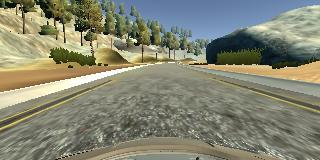
\includegraphics[scale = 1]{flipped_center_2017_12_21_20_06_58_582.jpg}
\caption{Flipped image}
\end{figure}

After the collection process I had 24,902 images. I preprocessed this data by normalizing and cropping 50 pixels off the top and 20 off the bottom of the image. I shuffled the data and set aside 20\% of the data for validation. I used this training data for training the model. The validation set helped determine if the model was over or under fitting. The ideal number of epochs was 5 as evidenced by the following graph. After 5 epochs, performance starts to get worse. I used an adam optimizer so that manually training the learning rate wasn't necessary.

\begin{figure}[h]
\centering
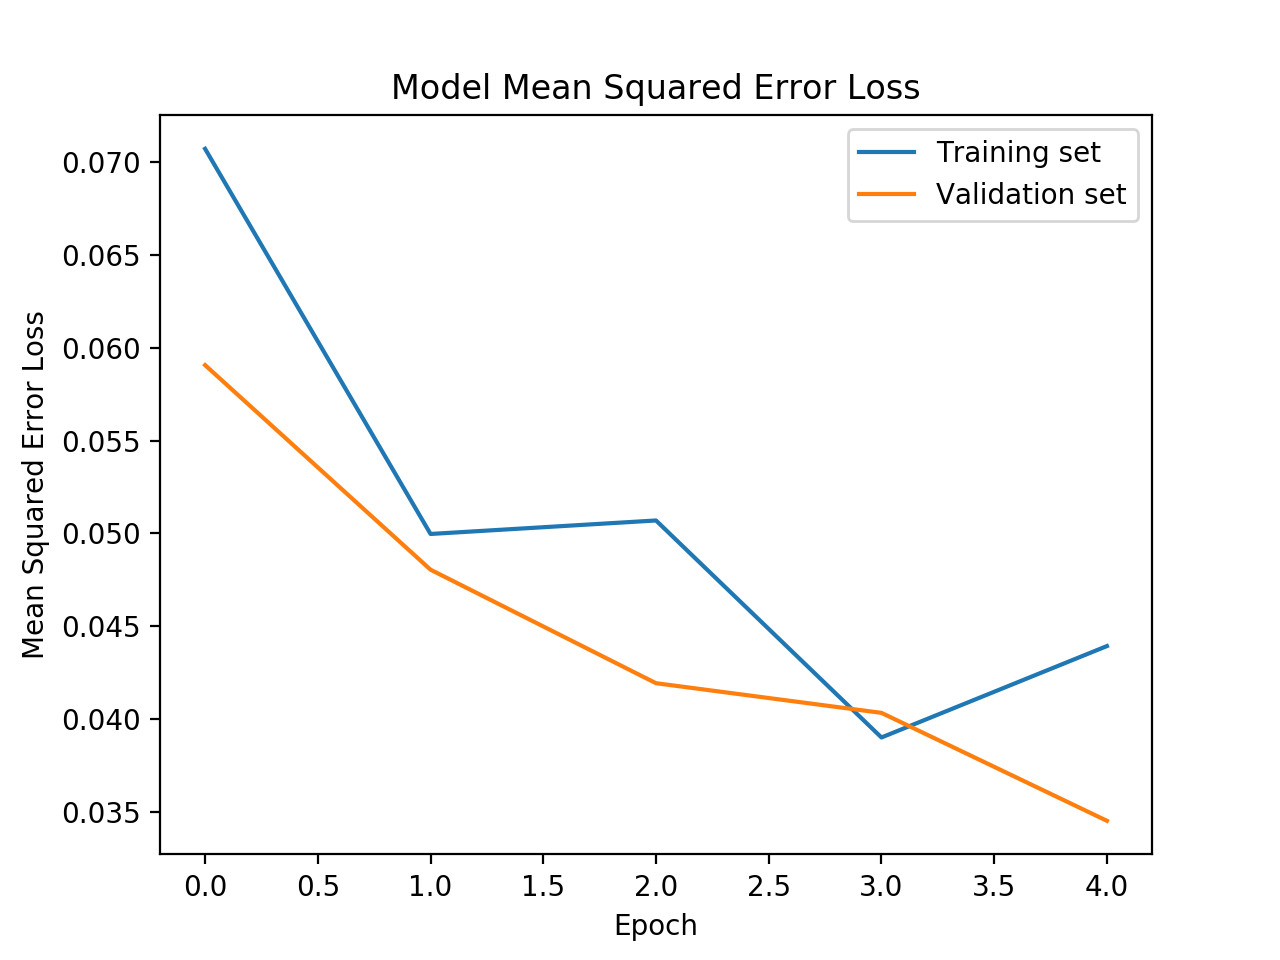
\includegraphics[scale = 1]{train_validation_loss.png}
\caption{Flipped image}
\end{figure}

[1] Y. LeCun, L. Bottou, Y. Bengio, and P. Haffner, "Gradient-Based Learning Applied to Document Recognition," \textit{Proc. IEEE}, vol.86, no. 11, pp. 2278-2324, Nov. 1998.
[2] Bojarski, Mariusz, et al. "End to end learning for self-driving cars." arXiv preprint arXiv:1604.07316 (2016).

\end{document}
